\documentclass{article}
\usepackage[utf8]{inputenc}

% Author: Ben Bloem-Reddy
%		  UBC
\usepackage[utf8]{inputenc}
\usepackage{verbatim}
\usepackage{titlesec}
\usepackage{fancyhdr}

%\usepackage[sorting=nyt,backend=biber,bibstyle=alphabetic,citestyle=alphabetic,giveninits=true]{biblatex}
\usepackage[backend=biber, natbib]{biblatex}

\def\coursename{STAT 550: Techniques of Statistical Consulting}
\def\shortcoursename{STAT 550}
\def\semester{Winter 2019/2020}

\setlength{\oddsidemargin}{0.0 in}
\setlength{\evensidemargin}{0.0 in} 
\setlength{\topmargin}{-0.6 in} 
\setlength{\textwidth}{6.5 in} 
\setlength{\textheight}{8.5 in}
\setlength{\headsep}{0.75 in} 
\setlength{\parindent}{0 in}
\setlength{\parskip}{0.1 in}


\titleformat*{\section}{\Large\bfseries}





\newcommand{\printtitle}{
    %\pagestyle{myheadings}
    \thispagestyle{plain}
    \pagenumbering{gobble}
    \newpage
    \noindent
    \begin{center}
        {\LARGE An Analysis on Commercial Real Estate Property Assessment and Property Tax in B.C.}
        \vskip 5mm
        {\large \begin{tabular}{cccc} Gian Carlo Di-Luvi & Mallory Flynn & Sophia Li & Vittorio Romaniello \end{tabular}} \\
        {\large STAT 550 Project Report} \\
        {\large April 2020} \\
        \vskip 5mm
        {\large Department of Statistics} \\
        {\large University of British Columbia}
    \end{center}
    
    \newpage

    \pagestyle{fancy}
    \pagenumbering{arabic}
    \fancyhf{}
    \lhead{\coursename}
    %\chead{\shortcoursename}
    \rhead{Di-Luvi, Flynn, Li, Romaniello}
    \cfoot{\thepage}
}
\usepackage{graphicx,amssymb,amsmath,amsthm,mathrsfs}
\usepackage{multirow,makeidx,algorithmic,algorithm}
\usepackage{mathtools}
\usepackage{enumitem}

\usepackage{float}
\floatplacement{figure}{h}
\usepackage{placeins}

\usepackage{dsfont}
\usepackage[table]{xcolor} % alternating row colors in tables

\usepackage{hyperref}
\usepackage{cleveref}
\usepackage{multirow}

\usepackage{subcaption}
% ADD YOUR CUSTOM NOTATION HERE

%% GCD %%

% set theory
\newcommand{\suchthat}{\, : \,} % Set such that
\newcommand{\given}{\, \mid \,}        % Conditional probability

% probability operators
\def\P{\bbP} %fundamental probability
\def\E{\bbE} %expectation
\newcommand{\convergence}[2]{\overset{#1}{\underset{#2}{\longrightarrow}}} %convergence in d,p,a.s.
\def\dconvergence{\overset{\mathrm{d}}{\longrightarrow}} % convergence in distribution
\def\pconvergence{\overset{p}{\longrightarrow}} % convergence in probability
\def\asconvergence{\overset{\mathrm{as}}{\longrightarrow}} % a.s. convergence

% stats operators
\newcommand{\SD}{\mathrm{SD}} %standard deviation
\newcommand{\Var}{\mathrm{Var}} % variance
\def\MLE{\mathrm{MLE}} %maximum likelihood extimator
\def\MSE{\mathrm{MSE}} %mean squared error

% stats distributions
\def\Bernoulli{\mathrm{Bernoulli}}
\def\Binom{\mathrm{Binomial}}
\def\Poisson{\mathcal{Poisson}}
\def\Geom{\mathcal{Geometric}}
\def\NegBinom{\mathrm{NegBinom}}
\def\Normal{\mathcal{N}}
\def\Gammadist{\mathrm{Gamma}}
\def\Beta{\mathrm{Beta}}
\def\Exp{\mathrm{Exp}}

% math operators
\DeclareMathOperator*{\argmax}{arg\,max}
\DeclareMathOperator*{\argmin}{arg\,min}
\def\d{\,\mathrm{d}} % for integration
\def\exp{\mathrm{exp}}
\newcommand{\floor}[1]{\left\lfloor #1 \right\rfloor} % floor function
\newcommand{\ceiling}[1]{\left\lceil #1 \right\rceil} % ceiling function

% matrix operators
\newcommand{\rank}{\mathrm{rank}}
\newcommand{\trace}{\mathrm{tr}}

%% End of GCD %%

% Author: Ben Bloem-Reddy
%		  UBC
%%
% full alphabets of different styles
%%

% bf series
\def\bfA{\mathbf{A}}
\def\bfB{\mathbf{B}}
\def\bfC{\mathbf{C}}
\def\bfD{\mathbf{D}}
\def\bfE{\mathbf{E}}
\def\bfF{\mathbf{F}}
\def\bfG{\mathbf{G}}
\def\bfH{\mathbf{H}}
\def\bfI{\mathbf{I}}
\def\bfJ{\mathbf{J}}
\def\bfK{\mathbf{K}}
\def\bfL{\mathbf{L}}
\def\bfM{\mathbf{M}}
\def\bfN{\mathbf{N}}
\def\bfO{\mathbf{O}}
\def\bfP{\mathbf{P}}
\def\bfQ{\mathbf{Q}}
\def\bfR{\mathbf{R}}
\def\bfS{\mathbf{S}}
\def\bfT{\mathbf{T}}
\def\bfU{\mathbf{U}}
\def\bfV{\mathbf{V}}
\def\bfW{\mathbf{W}}
\def\bfX{\mathbf{X}}
\def\bfY{\mathbf{Y}}
\def\bfZ{\mathbf{Z}}

% bb series
\def\bbA{\mathbb{A}}
\def\bbB{\mathbb{B}}
\def\bbC{\mathbb{C}}
\def\bbD{\mathbb{D}}
\def\bbE{\mathbb{E}}
\def\bbF{\mathbb{F}}
\def\bbG{\mathbb{G}}
\def\bbH{\mathbb{H}}
\def\bbI{\mathbb{I}}
\def\bbJ{\mathbb{J}}
\def\bbK{\mathbb{K}}
\def\bbL{\mathbb{L}}
\def\bbM{\mathbb{M}}
\def\bbN{\mathbb{N}}
\def\bbO{\mathbb{O}}
\def\bbP{\mathbb{P}}
\def\bbQ{\mathbb{Q}}
\def\bbR{\mathbb{R}}
\def\bbS{\mathbb{S}}
\def\bbT{\mathbb{T}}
\def\bbU{\mathbb{U}}
\def\bbV{\mathbb{V}}
\def\bbW{\mathbb{W}}
\def\bbX{\mathbb{X}}
\def\bbY{\mathbb{Y}}
\def\bbZ{\mathbb{Z}}

% cal series
\def\calA{\mathcal{A}}
\def\calB{\mathcal{B}}
\def\calC{\mathcal{C}}
\def\calD{\mathcal{D}}
\def\calE{\mathcal{E}}
\def\calF{\mathcal{F}}
\def\calG{\mathcal{G}}
\def\calH{\mathcal{H}}
\def\calI{\mathcal{I}}
\def\calJ{\mathcal{J}}
\def\calK{\mathcal{K}}
\def\calL{\mathcal{L}}
\def\calM{\mathcal{M}}
\def\calN{\mathcal{N}}
\def\calO{\mathcal{O}}
\def\calP{\mathcal{P}}
\def\calQ{\mathcal{Q}}
\def\calR{\mathcal{R}}
\def\calS{\mathcal{S}}
\def\calT{\mathcal{T}}
\def\calU{\mathcal{U}}
\def\calV{\mathcal{V}}
\def\calW{\mathcal{W}}
\def\calX{\mathcal{X}}
\def\calY{\mathcal{Y}}
\def\calZ{\mathcal{Z}}


%%%%%%%%%%%%%%%%%%%%%%%%%%%%%%%%%%%%%%%%%%%%%%%%%%%%%%%%%%
% text short-cuts
\def\iid{i.i.d.\ } %i.i.d.
\def\ie{i.e.\ }
\def\eg{e.g.\ }
\def\Polya{P\'{o}lya\ }
%%%%%%%%%%%%%%%%%%%%%%%%%%%%%%%%%%%%%%%%%%%%%%%%%%%%%%%%%%

% set theory/measure theory
\def\collection{\calC}
\newcommand{\sigalg}[1]{\mathcal{#1}}
\def\borel{\calB} %Borel sets
\def\sigAlg{\sigalg{H}} %sigma-algebra
\def\filtration{\calF} %filtration
\newcommand{\msblSpace}[1]{(#1,\sigalg{#1})}
\newcommand{\measSpace}[2][\mu]{(#2,\sigalg{#2},#1)}
\newcommand{\borelSpace}[1]{(#1,\borel(#1))}
\newcommand{\measFuncs}[1]{\sigalg{#1}^f}
\newcommand{\pbblSpace}{(\Omega,\sigAlg)}
\newcommand{\probSpace}[1][\bbP]{(\Omega,\sigAlg,#1)}

\def\leb{\lambda}

\def\finv{f^{-1}} % inverse
\def\ginv{g^{-1}} % inverse

% group theory
\def\grp{\calG} %group

% operators
% conditional expectation
\DeclarePairedDelimiterX\bigCond[2]{[}{]}{#1 \;\delimsize\vert\; #2}
\newcommand{\conditional}[3][]{\bbE_{#1}\bigCond*{#2}{#3}}
\def\Law{\mathcal{L}} %law; this is by convention in the literature
\def\indicator{\mathds{1}} % indicator function
%\def\1{{\mathbf 1}}
%\def\indicator{\1}

% binary relations
\def\condind{{\; \perp\!\!\!\perp \;}} %independence/conditional independence
\def\equdist{\stackrel{\text{\rm\tiny d}}{=}} %equal in distribution
\def\equind{\stackrel{\text{\rm\tiny ind}}{=}} %equal by independence
\def\equas{\stackrel{\text{\rm\tiny a.s.}}{=}} %equal almost surely
\def\simiid{\sim_{\mbox{\tiny iid}}} %sampled i.i.d

% common vectors and matrices
\def\onevec{\mathbf{1}}
\def\iden{\mathbf{I}} % identity matrix
\def\supp{\text{\rm supp}}

% misc
% floor and ceiling
%\DeclarePairedDelimiter{\ceilpair}{\lceil}{\rceil}
%\DeclarePairedDelimiter{\floor}{\lfloor}{\rfloor}
%\newcommand{\argdot}{{\,\vcenter{\hbox{\tiny$\bullet$}}\,}} %generic argument dot
%%%%%%%%%%%%%%%%%%%%%%%%%%%%%%%%%%%%%%%%%%%%%%%%%%%%%%%%%%


 
\usepackage{listings}
	\lstset{frame = single,
    		literate={á}{{\'a}}1
        			 {ã}{{\~a}}1
        			 {é}{{\'e}}1
        			 {ó}{{\'o}}1
        			 {í}{{\'i}}1
        			 {ñ}{{\~n}}1
        			 {¡}{{!`}}1
        			 {¿}{{?`}}1
        			 {ú}{{\'u}}1
                     {Á}{{\'A}}1
                     {É}{{\'E}}1
                     {Í}{{\'I}}1
                     {Ó}{{\'O}}1
                     {Ú}{{\'U}}1
} 

\definecolor{darkolivegreen}{rgb}{0.33, 0.42, 0.18}
\renewcommand{\lstlistingname}{Code}
\lstdefinestyle{R}{%
    %\captionsetup{labelformat=algocaption,labelsep=colon}
    mathescape=false,
    breaklines=true,
    frame=single,
    numbers=left, 
    numberstyle=\small,
    language=R,
    basicstyle=\scriptsize\ttfamily, 
    keywordstyle=\color{blue}\bf,
    xleftmargin=.04\textwidth,
    commentstyle=\color{darkolivegreen},
    stringstyle=\color{darkolivegreen},
    deletekeywords={mean, sd, start},
    morekeywords={TRUE, FALSE, seed}
}

\lstdefinestyle{regular}{%
    %\captionsetup{labelformat=algocaption,labelsep=colon}
    mathescape=false,
    breaklines=true,
    frame=single,
    numbers=left, 
    numberstyle=\small,
    language=R,
    basicstyle=\scriptsize\ttfamily, 
    keywordstyle=\color{black}\bf,
    xleftmargin=.04\textwidth
}
%-- 

\bibliography{../../ref/RealEstate.bib}


\begin{document}


\printtitle



\section*{Summary}
Property taxes are the single greatest operating expense for property owners in British Columbia, and mainly depend on two factors: property assessment---published each year in January---and municipal mill rates---published in April. Accurately projecting annual mill rates between January and April and future years' assessment values between May and December would allow businesses and individuals to budget for these expenses. For this purpose, multiple competing models are fitted based on a data set containing assessment values, mill rates, and other property information from 2016 to 2020 of over 200,000 properties. For predicting mill rates early in the year, a random forest regression model is found to be the most accurate. Likewise, another random forest regression model is also the most accurate for predicting future years' assessment values. Both models are incorporated in an interactive Shiny app that provides a straightforward user interface with a property-specific tax assessment.


\section{Introduction}
For property owners in British Columbia, property taxes are the single greatest operating expense. Mill rates are determined by individual municipalities and depend on a number of factors, including assessment values and municipal budgets.  While property assessments are published each year in January, municipal mill rates are not determined until April of the same calendar year, making it difficult for property owners to budget for this large expense.  Thus, accurately projecting the annual mill rates between the months of January and April and the next year's assessment values between May and December is a value-add to real estate consulting services. Furthermore, it also assists property owners in financial planning and fund allocation.  The objective of this written report is to build accurate statistical predictive models for both future municipal mill rates and property-specific assessment values. This will be done for tax class codes 1 (residential), 5 (light industrial), and 6 (commercial). Guided by the exploratory data analysis in Section \ref{section:eda}, several modeling techniques are presented in Section \ref{section:model}. Mill rate and assessment predictions using these models are available through a straightforward user interface via a Shiny app, which is discussed in the same section. Finally, Section \ref{section:conclusion} includes some concluding remarks.


\section{Statistical analysis} \label{section:analysis}

\subsection{Data} \label{sec:data}

\citet{s450-report} use the same dataset and offer a thorough description of the data in their analysis. In this report, however, all B.C. municipalities are included in analysis. The variables are summarised in Table \ref{table:variables}.  Missing mill rate values were imputed by using the average municipality mill rate for the corresponding year and tax class code. This is sensible because mill rates are constant across municipalities, and so a more complex imputation technique is not necessary.

An important feature of the data is that spatial relationships exist within municipalities for assessment values and between municipalities for mill rates.  In other words, it is not sensible to assume independence in neither assessment values nor mill rates between different properties because geographical location (and thus proximity) affects these variables. This significantly influences possible model choices as the independence assumption is required for several standard modeling techniques. Furthermore, the data set lacks appropriate spatial information that would allow for geographical variables to be taken into account.

\begin{table}[ht]
\centering
\rowcolors{2}{gray!20}{white}
\begin{tabular}{ll}
\rowcolor{gray!40}
\textbf{Variable}                & \textbf{Type}               \\ \hline
Mill rate                                                              & Continuous         \\
Total assessment                                                       & Continuous         \\
Total land assessment                                                  & Continuous         \\
Total improvement assessment & Continuous         \\
Tax class code                                                         & \begin{tabular}[c]{@{}l@{}}Categorical. \\ One of 1 (residential), 5 (industrial), 6 (commercial)\end{tabular}       \\
Municipality                                                           & Categorical        \\
Year & \begin{tabular}[c]{@{}l@{}}Discrete. \\ Values of 2016, 2017, 2018, and 2019\end{tabular} 
\end{tabular}
\caption{Brief description of the variables included in the data set.}
\label{table:variables}
\end{table}




\subsection{Exploratory data analysis} \label{section:eda}

The exploratory data analysis (EDA) further investigates aspects of the EDA done by \citet{s450-report}. Both assessment values and mill rates have right-skewed distributions, and so they were log-transformed for visualization purposes. A visual inspection of Figure \ref{fig:scatter_year} shows that mill rates differ drastically from tax class to tax class, with industrial properties having the highest mill rates. However, neither mill rates nor assessment values seem to vary much over time, which suggests that current values of these variables will be a good indicator of their (short-term) future values. Furthermore, there does not appear to be a clear relationship between assessment values and mill rates when tax class is taken into account---except in the residential tax class, where a slightly negative relationship is present between the logarithms of average municipal assessment values and municipal mill rates. This remains true when only taking into account values from 2020, as can be seen in Figure \ref{fig:scatter_2020}. 



\begin{figure}[ht]
\centering
\begin{subfigure}{.5\textwidth}
  \centering
  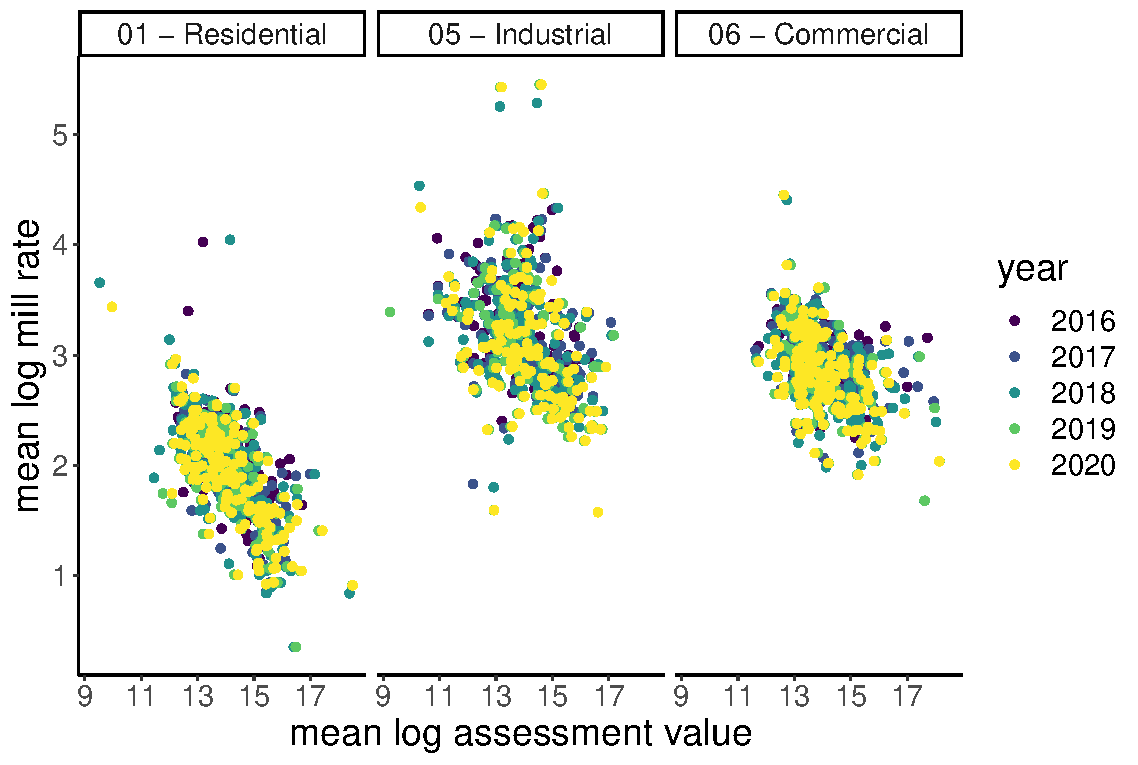
\includegraphics[width=.9\textwidth]{figures/1. scatter with year.pdf}
  \caption{Scatterplot with year in different colors.}
  \label{fig:scatter_year}
\end{subfigure}%
\begin{subfigure}{.5\textwidth}
  \centering
  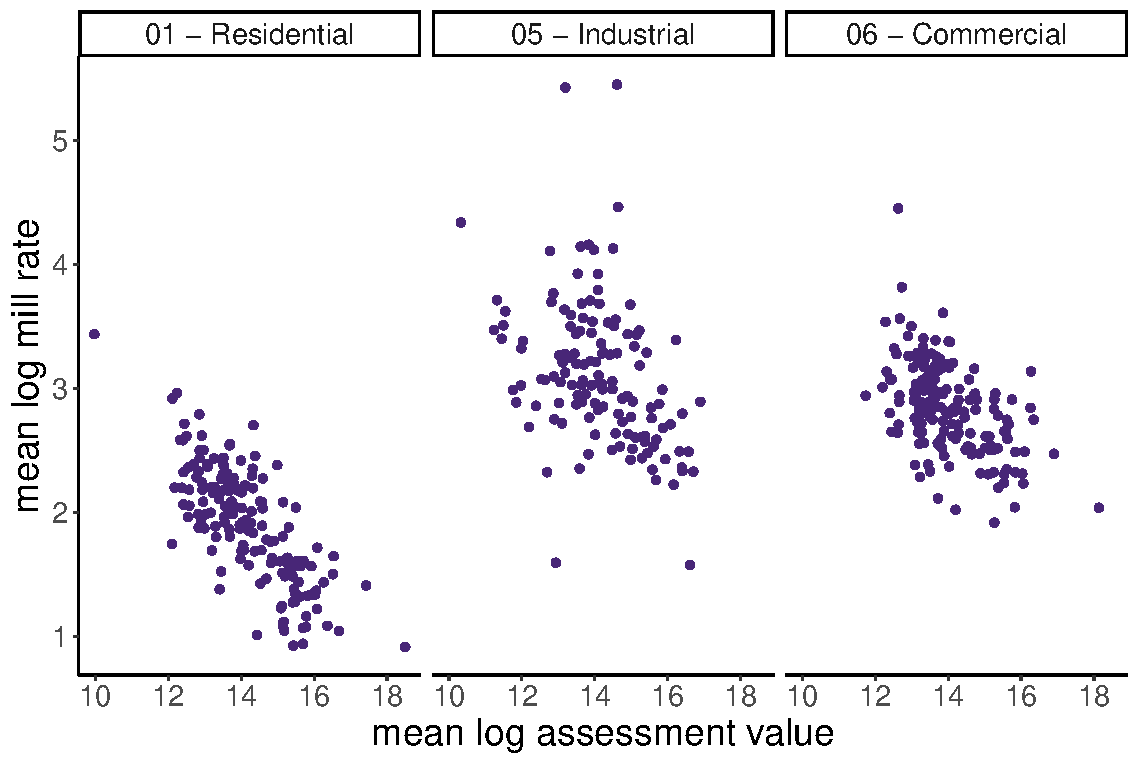
\includegraphics[width=.9\textwidth]{figures/2. scatter 2020 by municipality.pdf}
  \caption{Scatterplot only for 2020.}
  \label{fig:scatter_2020}
\end{subfigure}
\caption{Average log assessment values against log mill rates by municipality across the three different tax classes of interest.}
\label{fig:scatter}
\end{figure}


%\begin{figure}
%    \centering
%    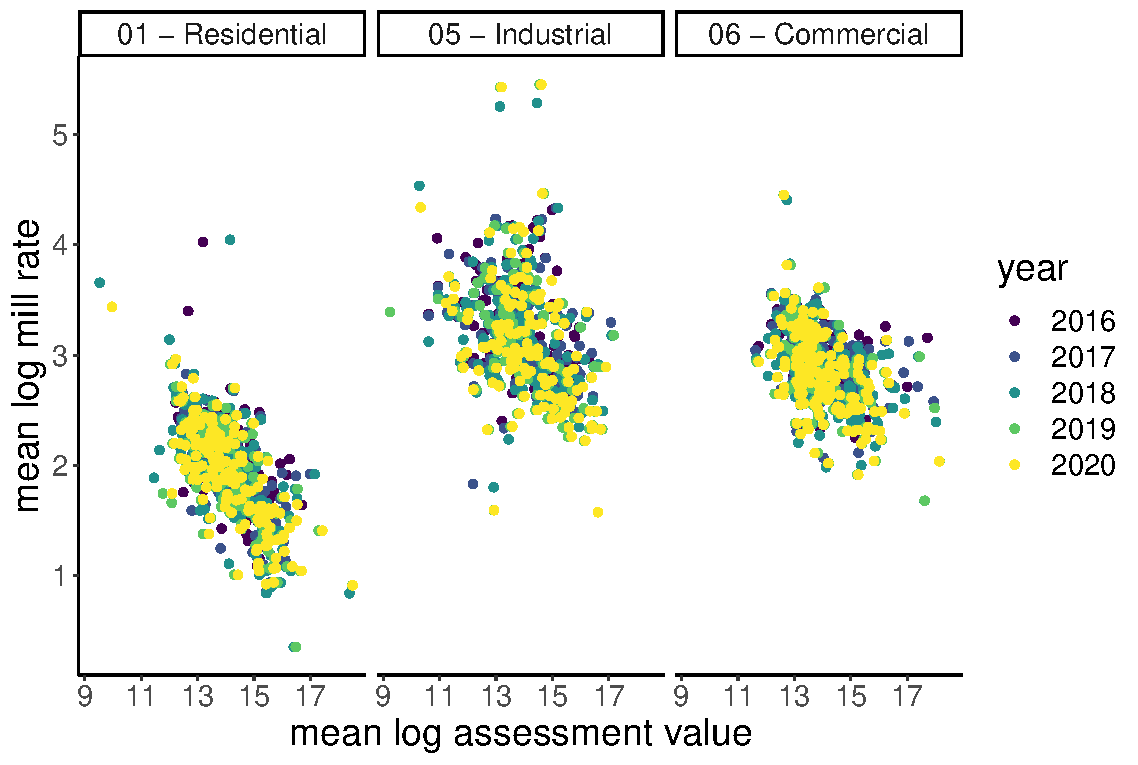
\includegraphics[scale=0.55]{figures/1. scatter with year.pdf}
%    \caption{Log assessment values against log mill rates across the three different tax classes of interest, with year in different colors.}
%    \label{fig:scatter_year}
%\end{figure}



The fact that mill rates remain relatively constant throughout the years is further verified in Figure \ref{fig:evolution_millrate}, where industrial properties are again seen to have the largest mill rates on average. However, Figure \ref{fig:evolution_assessment} suggests that assessment values do not follow this pattern. Municipality plays a role in a property's assessments, something taken into account in the modeling process.



Finally, Figure \ref{fig:violin} shows that the distributions of both mill rates and assessment values are indeed right-skewed (the values shown are in logarithmic scale), and further confirms the stark difference in mill rates between the three tax classes. Notably, Figure \ref{fig:violin_assessment} suggests that this difference is not present in assessment values, which indicates that tax class may not be that relevant for predicting future years' assessment values.


\begin{figure}[ht]
\centering
\begin{subfigure}{.5\textwidth}
  \centering
  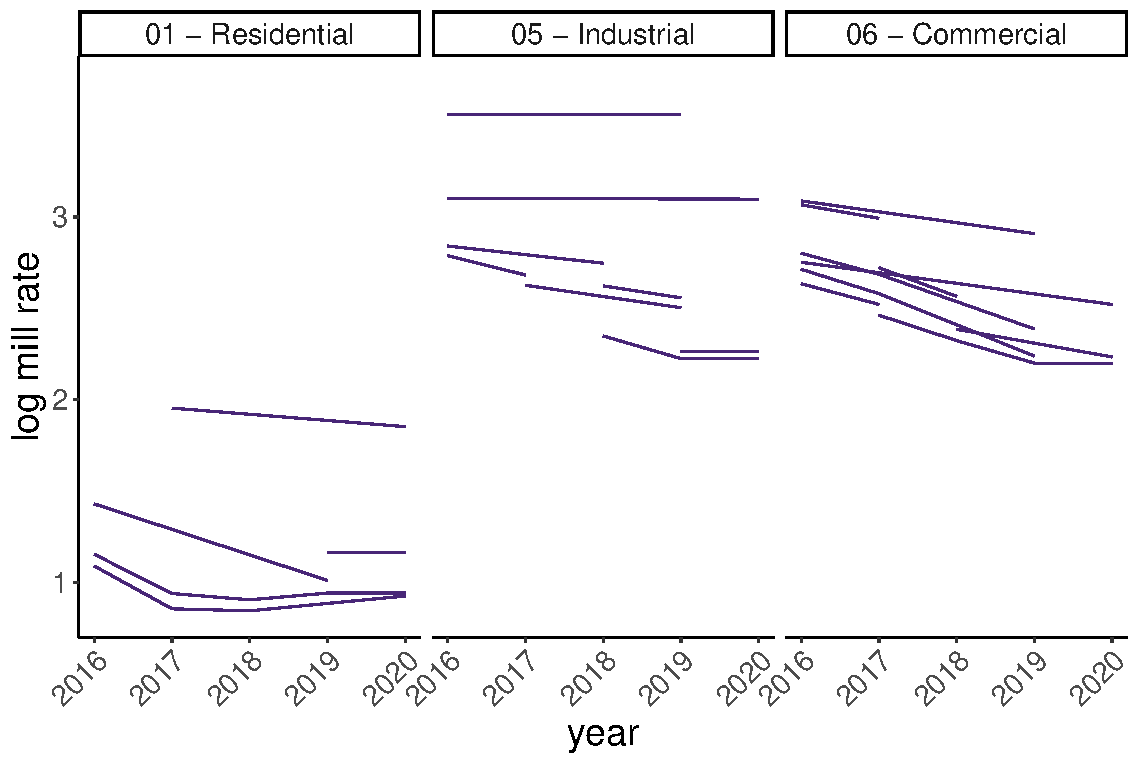
\includegraphics[width=.9\textwidth]{figures/6. mill rate evolution sample.pdf}
  \caption{Evolution of (log) mill rates.}
  \label{fig:evolution_millrate}
\end{subfigure}%
\begin{subfigure}{.5\textwidth}
  \centering
  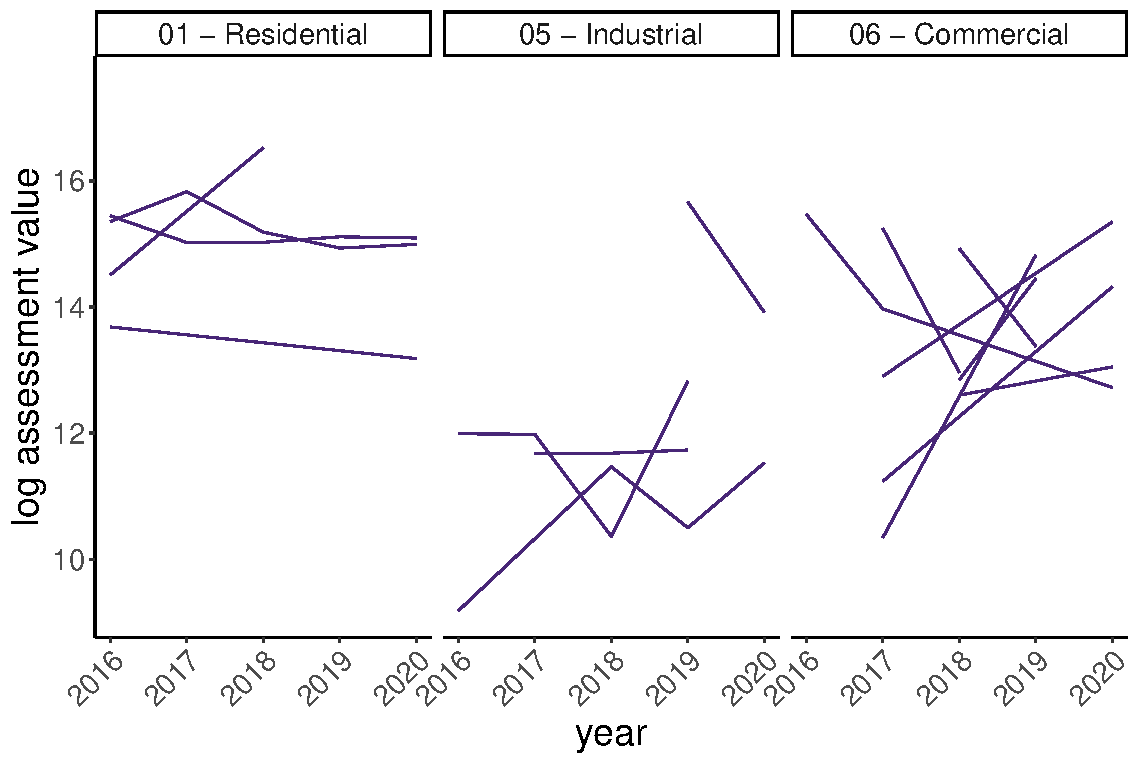
\includegraphics[width=.9\textwidth]{figures/6.1 assessment evolution sample.pdf}
  \caption{Evolution of (log) assessment values.}
  \label{fig:evolution_assessment}
\end{subfigure}
\caption{Evolution of target variables over the years for some randomly-selected properties.}
\label{fig:evolution}
\end{figure}



%\begin{figure}[ht]
%    \centering
%    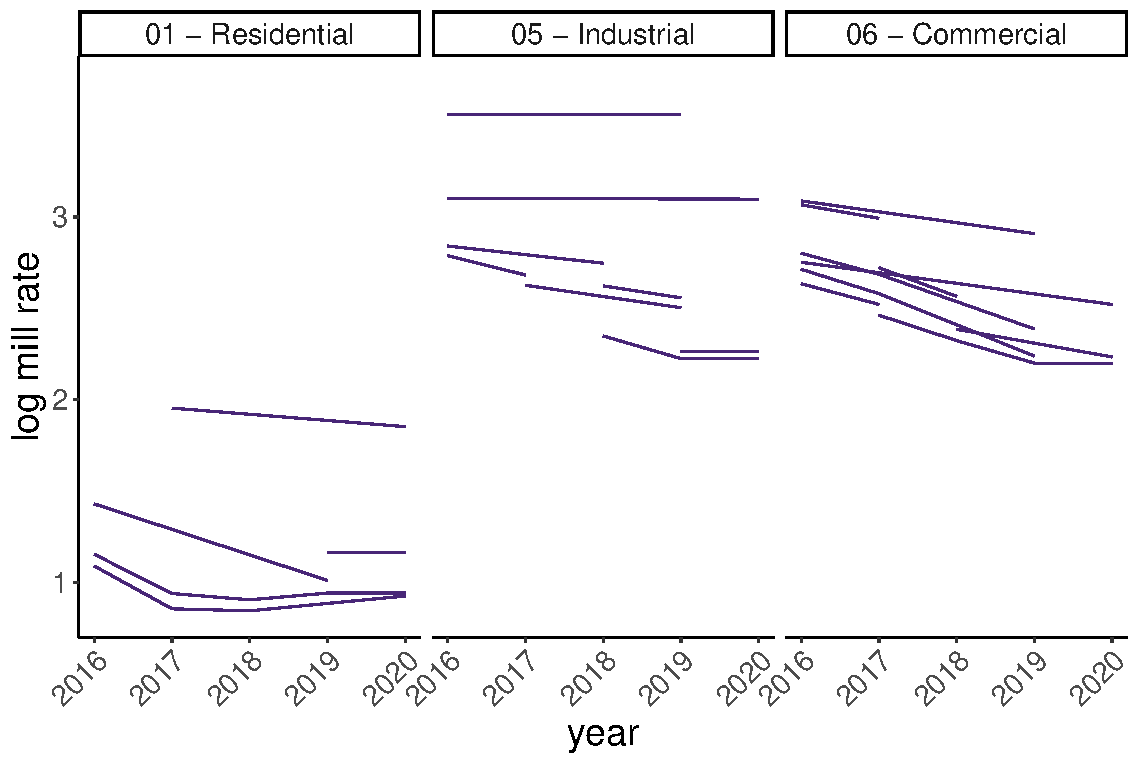
\includegraphics[scale=0.45]{figures/6. mill rate evolution sample.pdf}
%    \caption{Evolution of (log) mill rates over the years for some randomly-selected properties.}
%    \label{fig:rates_by_year}
%\end{figure}







\begin{figure}[ht]
\centering
\begin{subfigure}{.5\textwidth}
  \centering
  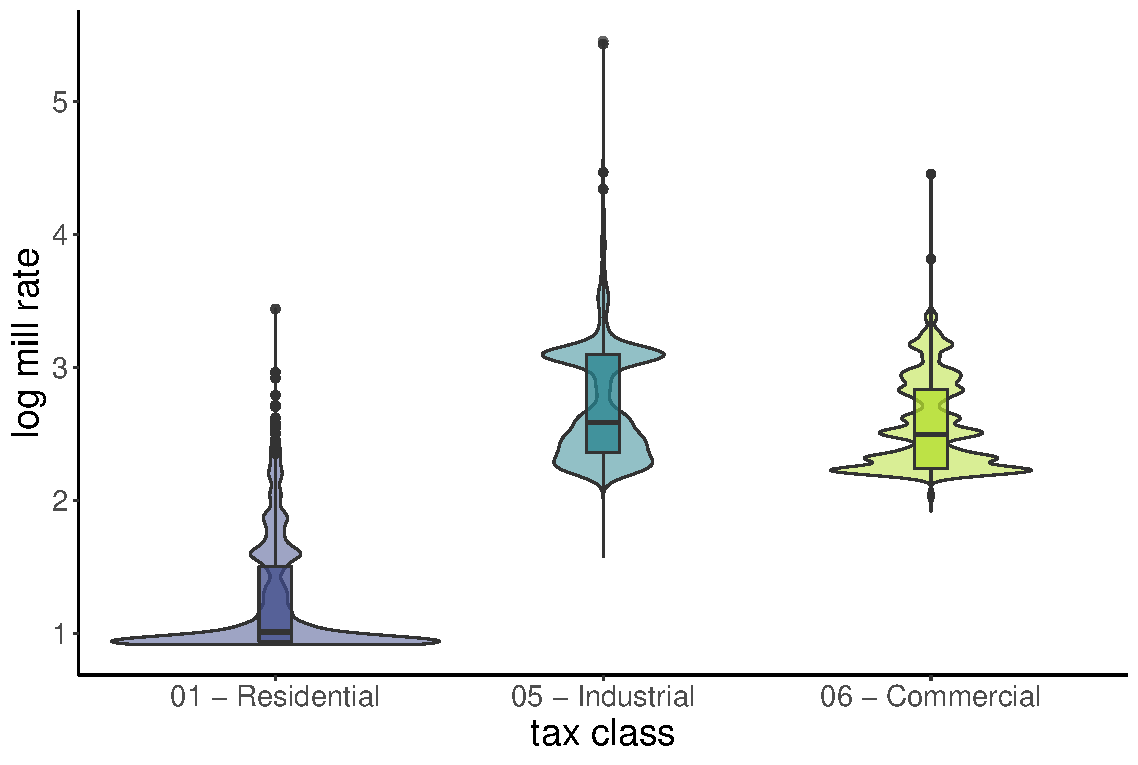
\includegraphics[width=.9\textwidth]{figures/7. violin mill rates.pdf}
  \caption{Distribution of (log) mill rates.}
  \label{fig:violin_millrate}
\end{subfigure}%
\begin{subfigure}{.5\textwidth}
  \centering
  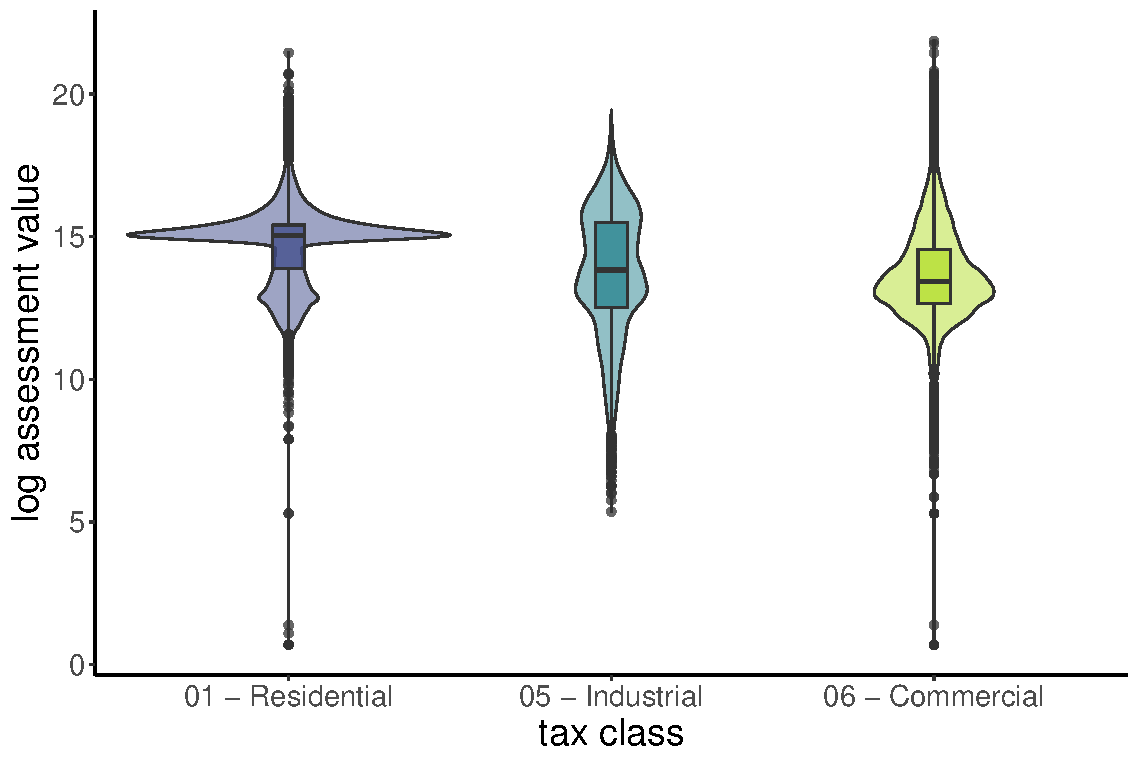
\includegraphics[width=.9\textwidth]{figures/7.1 violin assessment values.pdf}
  \caption{Distribution of (log) assessment values.}
  \label{fig:violin_assessment}
\end{subfigure}
\caption{Violin and boxplots of (log) mill rates and (log) assessment values of individual properties across the three tax classes of interest, taking into account only the year 2020.}
\label{fig:violin}
\end{figure}


%\begin{figure}[ht]
%    \centering
%    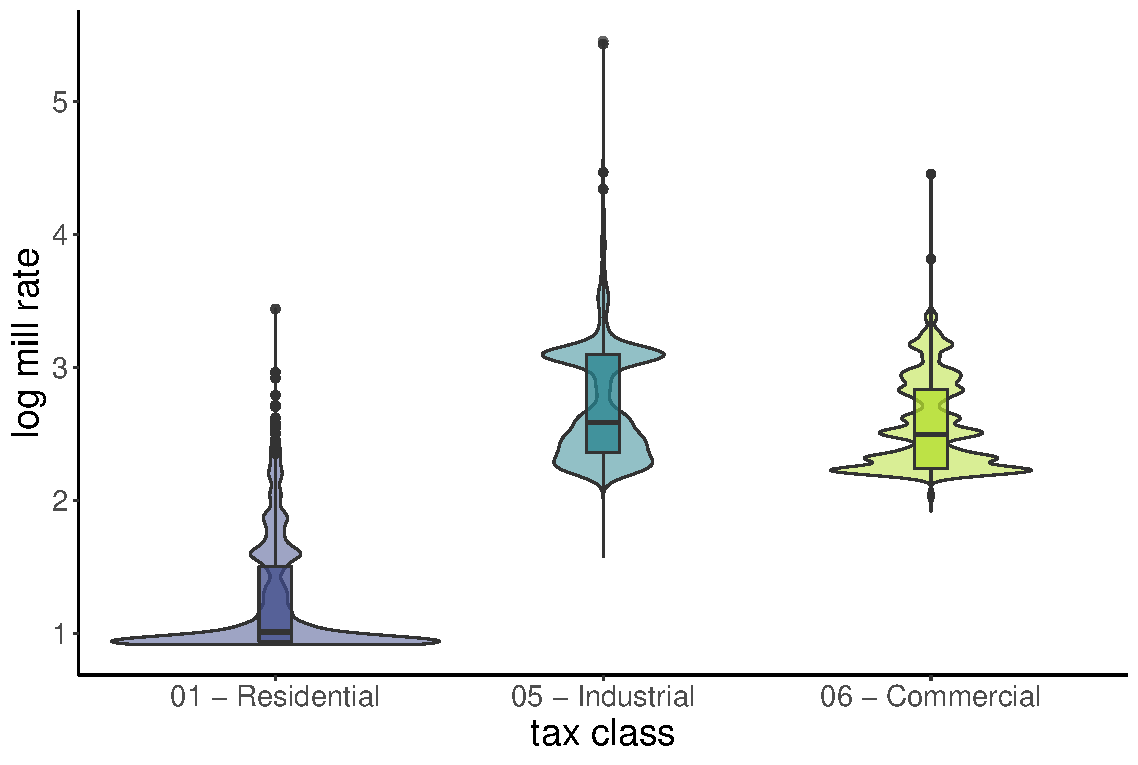
\includegraphics[scale=0.45]{figures/7. violin mill rates.pdf}
%    \caption{Violin and boxplots of (log) mill rates of individual properties across the three tax classes of interest, taking into account only the year 2020.}
%    \label{fig:violin}
%\end{figure}

\FloatBarrier


\subsection{Modeling} \label{section:model}

This section describes the models used to predict mill rate and assessment values. Each of the following models were trained on a subset of 75\% of the data and tested on the remaining 25\%.

\subsubsection{Random forest regression}

% Pick one of the two
The random forest (RF) algorithm is an ensemble learning method for classification and regression that operates by constructing numerous decision trees and choosing the majority class output (classification) or the average prediction (regression) given by the individual decision trees. Decision trees are trained on different samples (with replacement) of the data, and only a random subset of the covariates is used to define the split at each node, based on a recursive partitioning strategy. RF is preferred over a single decision tree as it overcomes the problem of over-fitting.  The following models were constructed using the 'randomForest' package in R \citep{rfpack}.

%%%
A RF model was fitted to predict mill rate using tax class, municipality, past years' mill rate, and current years' total assessment as independent variables. Another RF model was similarly constructed using next year's assessment value as the dependent variable, and municipality, current years' mill rate, tax class, and current years' total assessment as covariates. The number of trees used for both models was 500, and all 4 predictors were evaluated at each node for splitting. The percent of total variability explained is 96.38 \% for the mill rates model and 97.48 \% for the assessment values model. 

The importance of model covariates is indicated by a higher value of increase node purity (mean decrease accuracy). Municipality was deemed the most important variable in predicting mill rate (see Figure \ref{fig:4a}), followed by tax class and past year's mill rate. However, as shown in Figure  \ref{fig:4b}, current years' assessment value is the most important variable in predicting next years' assessment value, followed by municipality and mill rate.


\begin{figure}[ht]
\centering
\begin{subfigure}{.5\textwidth}
  \centering
  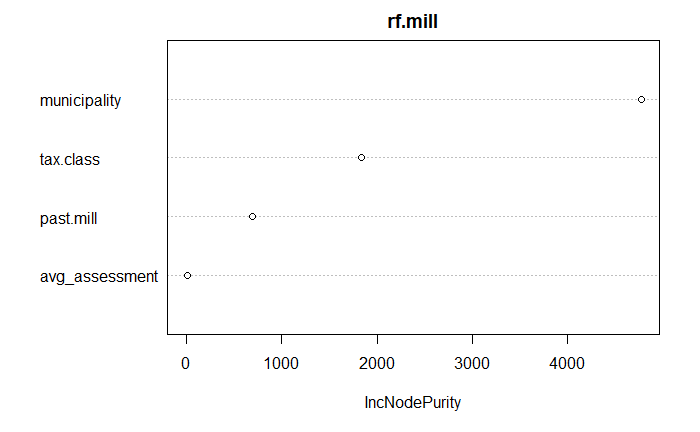
\includegraphics[width=.9\textwidth]{figures/nodepur.png}
  \caption{Variable importance plot for mill rates.}
  \label{fig:4a}
\end{subfigure}%
\begin{subfigure}{.5\textwidth}
  \centering
  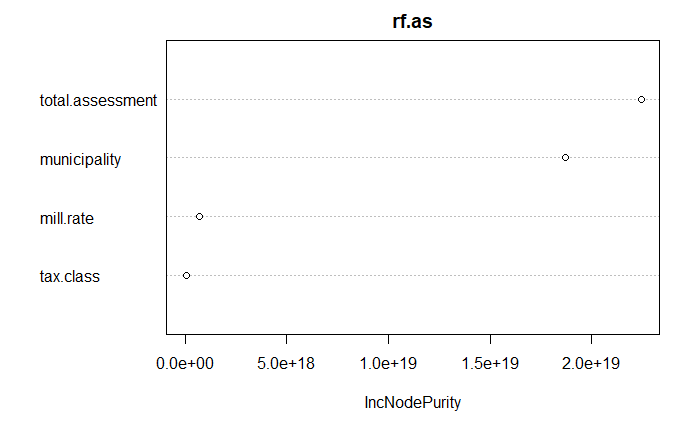
\includegraphics[width=.9\textwidth]{figures/asnodepur.png}
  \caption{Variable importance plot for assessment values.}
  \label{fig:4b}
\end{subfigure}
\caption{Variable importance plot based on increase in node purity for mill rate and total assessment value predictions.}
\label{fig:4}
\end{figure}

% Don't think it is necessary to mention bootstrapping, this is done automatically in RF.
Figure \ref{fig:5} shows the evaluation of the model's performance on a test dataset. The RF model tends to underestimate mill rates, probably due to the greater difficulty of the task. However, RF shows good performance in predicting next year's assessment values.

% Bagging (aggregate bootstrap) was implemented by the random forest algorithm and performance is shown in Figure \ref{fig:5}. Bagging uses bootstrapping---sampling the data with replacement---and aggregation---combining several model predictions to obtain the best prediction.  The accuracy of predicting mill rates is less optimal for higher mill rates.  However, overall, the prediction power of the random forest models are desirable, particularly for predicting next year's assessment value. 

\begin{figure}[ht]
\centering
\begin{subfigure}{.5\textwidth}
  \centering
  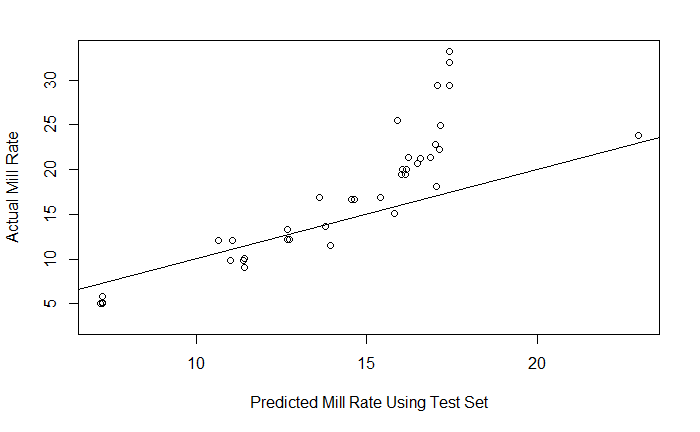
\includegraphics[width=.9\textwidth]{figures/bagmi.png}
  \caption{Performance for mill rates prediction.}
  \label{fig:5a}
\end{subfigure}%
\begin{subfigure}{.5\textwidth}
  \centering
  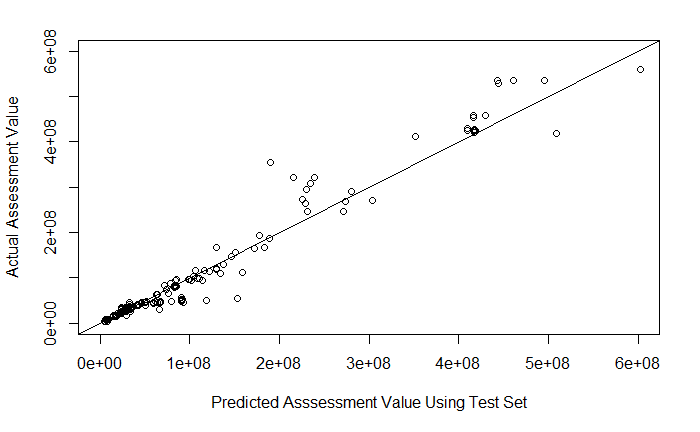
\includegraphics[width=.9\textwidth]{figures/bagas.png}
  \caption{Performance for assessment value prediction.}
  \label{fig:5b}
\end{subfigure}
\caption{Models' performance on test set.}
\label{fig:5}
\end{figure}
\FloatBarrier

\subsubsection{Mixed effects models and generalized estimating equation}
Since the data set contains repeated measurements for both municipalities and properties over the years, it is reasonable to consider a linear mixed effect model (LME) for predicting mill rates and assessment values. Both random slope and random intercept for each municipality are needed based on Figure \ref{fig:evolution_assessment}, which depicts different initial values and rates of change for both assessment values and municipal mill rates.  Based on the fixed effects shown in Figure \ref{fig:6b}, the direction of change in assessment values fluctuates over time. For example, assessment values increased from 2016 to 2017 but decreased from 2018 to 2020. The median municipal assessment value is positively associated with current mill rate, as is past year's mill rate (Figure \ref{fig:6a}). A negative relationship between mill rate and assessment values is observed in Figure \ref{fig:6b}, indicating that lower mill rates are associated with higher assessment values. 

\begin{figure}[ht]
\centering
\begin{subfigure}{.5\textwidth}
  \centering
  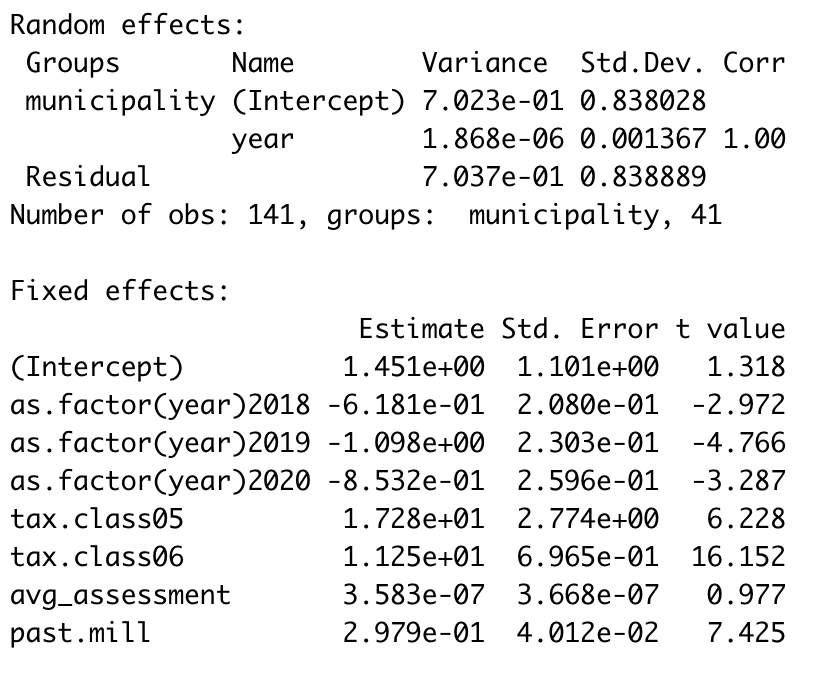
\includegraphics[width=.9\textwidth]{figures/lmemill.png}
  \caption{Summary output for predicting mill rates.}
  \label{fig:6a}
\end{subfigure}%
\begin{subfigure}{.5\textwidth}
  \centering
  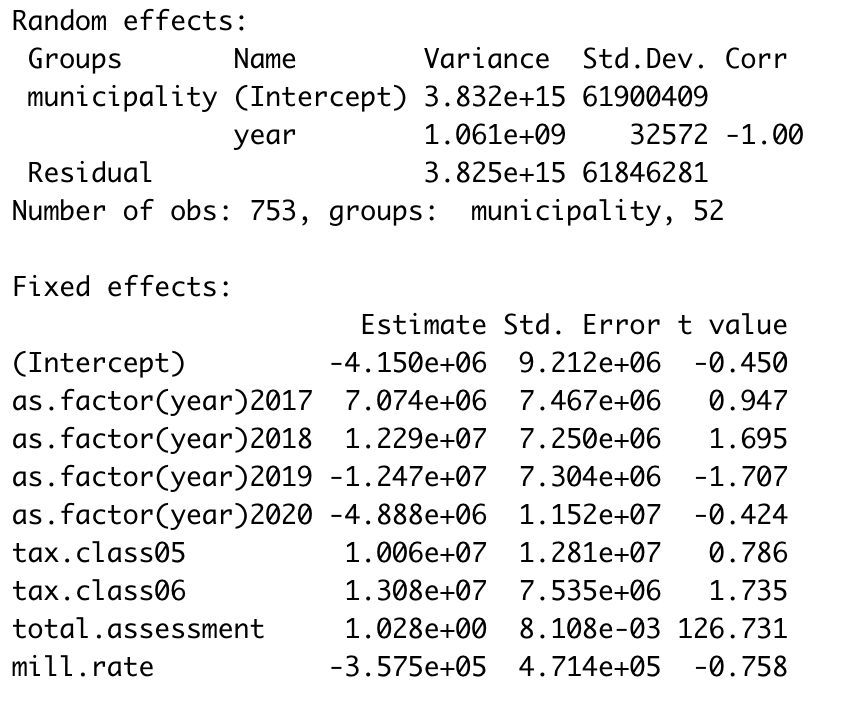
\includegraphics[width=.9\textwidth]{figures/lmeas.png}
  \caption{Summary output for predicting assessment values.}
  \label{fig:6b}
\end{subfigure}
\caption{Models summary output.}
\label{fig:6}
\end{figure}

\begin{figure}[ht]
\centering
\begin{subfigure}{.5\textwidth}
  \centering
  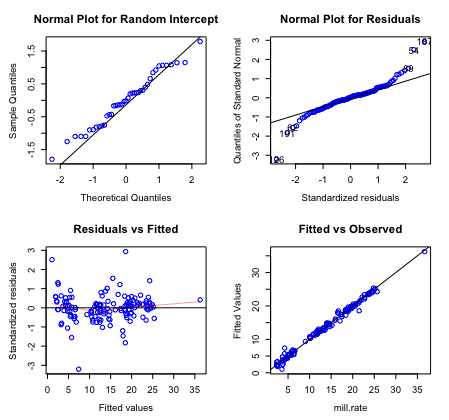
\includegraphics[width=.9\textwidth]{figures/diagmill.png}
  \caption{Diagnostics plots for LME model for mill rate.}
  \label{fig:7a}
\end{subfigure}%
\begin{subfigure}{.5\textwidth}
  \centering
  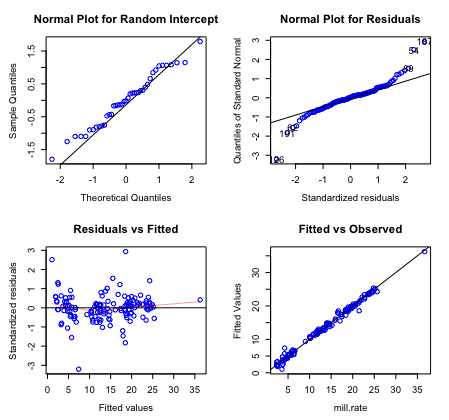
\includegraphics[width=.9\textwidth]{figures/diagas.png}
  \caption{Diagnostics plots for LME model for assessment values.}
  \label{fig:7b}
\end{subfigure}
\caption{Diagnostics plots.}
\label{fig:7}
\end{figure}

Unfortunately, the diagnostics plots verifying model assumptions are subpar for both LME models, as can be seen in Figure \ref{fig:7}. Residuals are not normally distributed, variance is heterogeneous, and random intercept is non-normal.  Thus it does not appear that an analysis using this type of model is appropriate for this data.


\subsubsection{Shiny app}

A straightforward user interface for making predictions using the RF models for mill rate and assessment values was built by way of a shiny app, which can be found in the GitHub repository \citep{gitrepo} or accessed on the web at {\color{blue} \underline{\url{https://malloryjflynn.shinyapps.io/STAT550_Real_Estate/}}}. 

The shiny app calculates predictions of the next years' mill rate or assessment value under the `Estimate' tab of the main panel.  This can be done using either a Property Identifier Code (PIC) or user inputs for municipality, tax class code, and previous year's mill rate (mill rate predictions) or current assessment value (assessment value predictions).  To provide the user with a broader view of the trend in mill rate for the municipality selected, a plot of the mill rate for that municipality over the years (2016 - 2020) is visible under the `Plot' tab of the main panel.  When predicting assessment value using a PIC, a plot of the assessment value for that property over time will be displayed alternatively.


\section{Conclusions} \label{section:conclusion}

In this report we built models to predict mill rate and assessment value for properties in British Columbia's municipalities. Random forest was found to be the best fitting model, although it tended to overestimate mill rate predictions. In addition to this, we incorporated the predictive models in a shiny app that allows a user to perform predictions given a set of inputs and to visualize trends in mill rate and assessment value.

The main limitation of our analysis lies in the fact that the models assume independence of the data. However, as was argued in Section \ref{sec:data}, mill rates and assessment values are highly dependent on spatial information. An attempt to obtain the properties' spatial information was made by transforming the addresses into spatial coordinates using an open source geocoding system provided by the British Columbia Government (see the documentation of \citet{geopy}). However, the open source geocoding system did not recognize some of the addresses in the dataset and provided incorrect coordinates for a large number of properties.  Therefore it is recommended that (1) addresses be formatted according to the standards required by the B.C. government, or (2) a private geocoding system that may be able to find addresses using the current format in the data is used. Provided spatial information is available, several model alternatives (e.g. factor models) could be tested to improve prediction accuracy, which take spatial information into account.


%%%% appendix and bibliography
\newpage
\printbibliography

\clearpage
\appendix
\section*{Appendix}


\section{EDA code}


\begin{lstlisting}[style=R, caption={Code used for the exploratory data analysis.}, captionpos=b]
# preamble ####
library(tidyverse)
library(readr)
library(readxl)
library(ggplot2)
ggplot2::theme_set(theme_classic())
library(viridis)

# data wrangling ####

# data import
columnnames <- readxl::read_xlsx("colnames.xlsx") %>% 
  colnames()

real.estate_full <- readr::read_csv("2016 - 2020 Raw.csv",
                                    na = c("", "NA", "NULL", "NULL_1"),
                                    col_names = columnnames,
                                    col_types = "ciccccccccccccccdddddiicccddddc")
# data wrangling

# assessments by PIC and year
assessments <- real.estate_full %>% 
  dplyr::select(PIC, Year, # relevant variables
                AssessedValueAmt, AssetTypeDesc) %>% 
  dplyr::rename(year = Year,
                assessment = AssessedValueAmt,
                assessment.type = AssetTypeDesc) %>% 
  dplyr::group_by(PIC, year, assessment.type) %>% 
  dplyr::summarise(assessment = sum(assessment)) %>% 
  dplyr::ungroup() %>% 
  tidyr::spread(assessment.type, assessment) %>% 
  dplyr::rename(improvement.assessment = Improvement,
                land.assessment = Land) %>% 
  dplyr::select(PIC, year, improvement.assessment, land.assessment) %>% 
  dplyr::mutate(total.assessment = improvement.assessment + land.assessment)


re <- real.estate_full %>% 
  dplyr::select(PIC, Year, AddressAssessorMunicipalityDesc, # relevant variables
                TaxClassCode, TaxOwingAmountTotalCalculated, TaxClassTaxRate) %>% 
  dplyr::rename(year = Year,
                municipality = AddressAssessorMunicipalityDesc, # human-readable names
                tax.class = TaxClassCode,
                tax = TaxOwingAmountTotalCalculated,
                mill.rate = TaxClassTaxRate) %>% 
  dplyr::filter(tax.class %in% c("01", "05", "06")) %>%  # relevant values for tax class
  dplyr::distinct() %>% 
  dplyr::left_join(assessments, by = c("PIC" = "PIC", "year" = "year")) # add assessment


# data viz ####
# tax classes dictionary
tax.classes <- as_labeller(c(
  `01` = "01 - Residential",
  `05` = "05 - Industrial",
  `06` = "06 - Commercial"
))


# facet scatter plots with year
re %>% 
  dplyr::select(-PIC) %>% 
  dplyr::filter(!is.na(total.assessment), !is.na(mill.rate)) %>% 
  dplyr::group_by(year, municipality, tax.class) %>% 
  dplyr::summarise(total.assessment = mean(total.assessment), mill.rate = mean(mill.rate)) %>% 
  ggplot(aes(x = log(total.assessment), y = log(mill.rate), color = factor(year))) +
  geom_point() +
  facet_wrap(.~tax.class, labeller = tax.classes) +
  labs(x = "log assessment value",
       y = "log mill rate",
       color = "year") +
  scale_color_viridis_d() +
  theme(text = element_text(size = 18))
ggsave("RealEstate/src/eda - s550/plots/1. scatter with year.pdf")
ggsave("RealEstate/src/eda - s550/plots/1. scatter with year.png")


# facet scatter plots for 2020 by municipality
re %>% 
  dplyr::filter(year == 2020) %>% 
  dplyr::select(-PIC, -year) %>% 
  dplyr::filter(!is.na(total.assessment), !is.na(mill.rate)) %>% 
  dplyr::group_by(municipality, tax.class) %>% 
  dplyr::summarise(total.assessment = mean(total.assessment), mill.rate = mean(mill.rate)) %>% 
  ggplot(aes(x = log(total.assessment), y = log(mill.rate))) +
  geom_point(color = viridis(20)[3]) +
  facet_wrap(.~tax.class, labeller = tax.classes) +
  labs(x = "log assessment value",
       y = "log mill rate") +
  theme(text = element_text(size = 18))
ggsave("RealEstate/src/eda - s550/plots/2. scatter 2020 by municipality.pdf")
ggsave("RealEstate/src/eda - s550/plots/2. scatter 2020 by municipality.png")



# facet line trends sample of 10
  re %>% 
    dplyr::select(-PIC) %>% 
    dplyr::filter(!is.na(total.assessment), !is.na(mill.rate)) %>% 
    dplyr::group_by(year, tax.class) %>% 
    dplyr::sample_n(size = 10) %>% 
    dplyr::ungroup() %>% 
    dplyr::group_by(year, tax.class, municipality) %>% 
    dplyr::summarise(total.assessment = mean(total.assessment), mill.rate = mean(mill.rate)) %>% 
    ggplot(aes(x = year, y = log(mill.rate), group = municipality)) +
    geom_line(color = viridis(20)[3]) +
    facet_wrap(.~tax.class, labeller = tax.classes) + 
    #scale_color_viridis_d() +
    #theme(legend.position = "none") +
    labs(x = "year",
         y = "log mill rate") +
    theme(text = element_text(size = 18),
          axis.text.x = element_text(angle = 45, hjust = 1))
  ggsave("RealEstate/src/eda - s550/plots/6. mill rate evolution sample.pdf")
  ggsave("RealEstate/src/eda - s550/plots/6. mill rate evolution sample.png")
  
    # facet line trends sample of 10 assessment
  re %>% 
    dplyr::select(-PIC) %>% 
    dplyr::filter(!is.na(total.assessment), !is.na(mill.rate)) %>% 
    dplyr::group_by(year, tax.class) %>% 
    dplyr::sample_n(size = 10) %>% 
    dplyr::ungroup() %>% 
    dplyr::group_by(year, tax.class, municipality) %>% 
    dplyr::summarise(total.assessment = mean(total.assessment), mill.rate = mean(mill.rate)) %>% 
    ggplot(aes(x = year, y = log(total.assessment), group = municipality)) +
    geom_line(color = viridis(20)[3]) +
    facet_wrap(.~tax.class, labeller = tax.classes) + 
    #scale_color_viridis_d() +
    #theme(legend.position = "none") +
    labs(x = "year",
         y = "log assessment value") +
    theme(text = element_text(size = 18),
          axis.text.x = element_text(angle = 45, hjust = 1))
  ggsave("RealEstate/src/eda - s550/plots/6.1 assessment evolution sample.pdf")
  ggsave("RealEstate/src/eda - s550/plots/6.1 assessment evolution sample.png")
  
  
  
  
  # violin plots of mill rates accross tax classes, for 2020
  re %>%  
    dplyr::filter(!is.na(total.assessment), !is.na(mill.rate), year == 2020) %>% 
    dplyr::group_by(PIC, tax.class) %>% 
    dplyr::summarise(total.assessment = mean(total.assessment), mill.rate = mean(mill.rate)) %>% 
    ggplot(aes(x = tax.class, y = log(mill.rate), fill = tax.class)) +
    geom_violin(alpha = 0.5, width = 1) +
    geom_boxplot(alpha = 0.75, width = 0.1) +
    labs(x = "tax class",
         y = "log mill rate") +
    #scale_fill_viridis_d(begin=0, end=1) +
    scale_fill_manual(values = c("#3E4A89FF", "#26828EFF","#B4DE2CFF" )) +
    theme(legend.position = "none") +
    scale_x_discrete(labels = c("01 - Residential", "05 - Industrial", "06 - Commercial")) +
    theme(text = element_text(size = 18))
  ggsave("RealEstate/src/eda - s550/plots/7. violin mill rates.pdf")
  ggsave("RealEstate/src/eda - s550/plots/7. violin mill rates.png")
  
  
  # violin plots of assessment values accross tax classes, for 2020
  re %>%  
    dplyr::filter(!is.na(total.assessment), !is.na(mill.rate), year == 2020) %>% 
    dplyr::group_by(PIC, tax.class) %>% 
    dplyr::summarise(total.assessment = mean(total.assessment), mill.rate = mean(mill.rate)) %>% 
    ggplot(aes(x = tax.class, y = log(total.assessment), fill = tax.class)) +
    geom_violin(alpha = 0.5, width = 1) +
    geom_boxplot(alpha = 0.75, width = 0.1) +
    labs(x = "tax class",
         y = "log assessment value") +
    #scale_fill_viridis_d(begin=0, end=1) +
    scale_fill_manual(values = c("#3E4A89FF", "#26828EFF","#B4DE2CFF" )) +
    theme(legend.position = "none") +
    scale_x_discrete(labels = c("01 - Residential", "05 - Industrial", "06 - Commercial")) +
    theme(text = element_text(size = 18))
  ggsave("RealEstate/src/eda - s550/plots/7.1 violin assessment values.pdf")
  ggsave("RealEstate/src/eda - s550/plots/7.1 violin assessment values.png")
\end{lstlisting}

\section{Modelling code}


\begin{lstlisting}[style=R, caption={Code used for the modeling.}, captionpos=b]
# preamble

suppressPackageStartupMessages(library(randomForest))
suppressPackageStartupMessages(library(tidyverse))
suppressPackageStartupMessages(library(lme4))
suppressPackageStartupMessages(library(ROCR))
suppressPackageStartupMessages(library(predictmeans))


###########################
# data prep
dat <- readr::read_delim("test_train_data.txt", delim = ",", col_types = "ciccdddddc")
dat$municipality <- as.factor(dat$municipality)
dat$tax.class <- as.factor(dat$tax.class)

factors_tbl = dat %>% 
  group_by(municipality) %>% 
  count(name="mun_count", sort = TRUE) %>% 
  ungroup() %>% 
  mutate(perc = mun_count/sum(mun_count),
         cum_perc = cumsum(perc)) %>% 
  arrange(desc(mun_count)) %>% 
  mutate(rank = row_number(),
         municipality = fct_reorder(municipality, rank)) %>% 
  mutate(col_municipality = fct_collapse(municipality, other = levels(municipality)[-c(1:52)])) %>% 
  select(municipality, col_municipality)


med_assessment_by_municipality = dat %>% 
  left_join(factors_tbl) %>% 
  select(-c(municipality)) %>% 
  rename(municipality = col_municipality) %>% 
  filter(test.train == "train") %>% 
  group_by(municipality, tax.class, year) %>% 
  mutate(med_assessment = median(total.assessment, na.rm=TRUE)) %>% 
  select(municipality, year, tax.class, med_assessment) %>% 
  distinct(municipality, .keep_all = T)

dat_mill <- dat %>% 
  left_join(factors_tbl) %>% 
  select(-c(municipality)) %>% 
  rename(municipality = col_municipality) %>% 
  left_join(med_assessment_by_municipality) %>% 
  group_by(PIC) %>% 
  mutate(next.assess = lead(med_assessment, order_by = year),
         past.mill = lag(mill.rate, order_by = year)) %>%
  arrange(PIC) %>% 
  group_by(municipality, year) %>% 
  mutate(n.prop = n()) %>% 
  arrange(desc(n.prop)) %>% 
  distinct(municipality, .keep_all = T) %>% 
  select(-c(tax, improvement.assessment, land.assessment, total.assessment))

dat_as <- dat %>% 
  left_join(factors_tbl) %>% 
  select(-c(municipality)) %>% 
  rename(municipality = col_municipality) %>% 
  group_by(PIC) %>% 
  arrange(year) %>% 
  mutate(next.assess = lead(total.assessment, order_by = year),
         past.mill = lag(mill.rate, order_by = year)) %>% 
  group_by(municipality) %>% 
  top_n(25, wt = total.assessment) %>% 
  arrange(municipality)

train_mill <- dat_mill %>%  filter(test.train == "train")
test_mill <- dat_mill %>%  filter(test.train == "test")
train_as <- dat_as %>%  filter(test.train == "train")
test_as <- dat_as %>%  filter(test.train == "test")

####################################
# Random Forest
set.seed(0)

rf.mill <- randomForest(
  mill.rate ~  tax.class + municipality + med_assessment + past.mill, na.action = na.omit, mtry = 4,
  data=train_mill, ntree=500
)

save(rf.mill, file = "rf.mill.rda")

#Evaluate variable importance
importance(rf.mill)
varImpPlot(rf.mill)

rf.as <- randomForest(
  next.assess ~ tax.class + municipality + total.assessment + mill.rate, na.action = na.omit,mtry = 4,
  data=train_as
)

save(rf.as, file = "rf.as1.rda")
importance(rf.as)
varImpPlot(rf.as)

yhat.bag <- predict(rf.mill,newdata=test_mill)
plot(yhat.bag, test_mill$mill.rate, xlab="Predicted Mill Rate Using Test Set", ylab="Actual Mill Rate")
abline(0,1)

yhat.bag1 <- predict(rf.as,newdata=test_as)
plot(yhat.bag1, test_as$next.assess, xlab="Predicted Asssessment Value Using Test Set", ylab="Actual Assessment Value", ylim=c(0, 10e8))
abline(0,1)

################################
# Linear Mixed Effects Model

# both random slope and random intercept
# different rate of change of assessment value and mill rate as well as initial assessment value and mill rate for each municipality 

lme.mill <- lmer(mill.rate ~ 1+ (1+year|municipality) + as.factor(year) + tax.class  + avg_assessment + past.mill, data = train_mill)

summary(lme.mill)

lme.as <- lmer(next.assess ~ 1+ (1+year|municipality) + as.factor(year) + tax.class + total.assessment + mill.rate, data = train_as)

summary(lme.as)

# check assumptions of lme

# Homogeneity of Variance
residplot(lme.mill)
residplot(lme.as)
\end{lstlisting}

\section{Shiny app code}


\begin{lstlisting}[style=R, caption={Code used for the Shiny app.}, captionpos=b]

#global.R file

library(shiny)
library(readr)
library(ggplot2)
library(dplyr)
library(DT)
library(tidyr)
library(shinyjs)
library(randomForest)

#PIC used for some testing
# CA-BC-200-001019632060000


# for bookmarking button
enableBookmarking("url")

# read data
dat <- readr::read_delim("test_train_data.txt", 
                         delim = ",", col_types = "ciccdddddf")

# creates dataset with only the top 52 municipalities
counts <- dat %>% 
  count(municipality, sort = TRUE)

datshort <- dat %>% 
  filter(municipality %in% counts$municipality[1:52])


# load dataset used for rf.mill
rfdat <- readRDS("rf_data.rds")

# create dataset used for rf.as
asdat <- readRDS("as_data.rds")
  
##################################
#################################
# ui.R file


# Mallory - STAT 550 2020###
# This is the user interface version of the shiny app

library(shinythemes)
library(png)

ui <- fluidPage(theme = shinytheme("cerulean"), #maybe journal theme?

                # header
                div(id = "headerSection",
                    h2("BC Mill Rate & Assessment Value Predictions"),
                    
                    span(
                      style = "font-size: 1em",
                      # authors
                      span("Created by "),
                      a("Gian Carlo Diluvi, Vittorio Romaniello, Sophia Li & Mallory Flynn",
                        href = "https://www.stat.ubc.ca"),
                      HTML("&bull;"),
                      # date
                      span("April 2020"),
                      HTML("&bull;"),
                      # Shiny app code link
                      span("Code"),
                      a("on GitHub", 
                        href = "https://github.com/STAT450-550/RealEstate/tree/master/src/shiny_app"),
                    )
                ),
                br(),
                br(),
                
                # all content goes here, and is hidden initially until the page fully loads
                sidebarLayout(
                  sidebarPanel(
                    # tabsetPanel(
                    #   tabPanel("User Inputs",        
                    
                    # Only show the following for assessment predictions:
                    # Use PIC?
                    checkboxInput("picInput", "Use PIC?", value = FALSE),
                    selectInput("typeInput", "Estimate Type",
                                c("Select", "Assessment Value", "Mill Rate"),
                                selected = "Select"),
                                     
                    # If using PIC:
                    conditionalPanel("input.picInput",
                                     textInput("identInput", "PIC:", placeholder = NULL)),
                                     
                    # If PIC is not available:
                    conditionalPanel("!input.picInput",
                                     
                                     # for municipality
                                     selectInput("municipalityInput", "Municipality:", 
                                                 c("-",sort(unique(datshort$municipality))),
                                                 selected = "-"),
                                                     
                                     # for Tax Class code
                                     selectInput("taxclassInput", "Tax Class Code:",
                                                 c("-",sort(unique(dat$tax.class))),
                                                 selected = "-"),
                                     
                                     #conditional input for estimate type
                                     conditionalPanel("input.typeInput == 'Assessment Value'",
                                                      numericInput("assessmentInput",
                                                                   "Current Assessment Value:",
                                                                   value = 70000000, 
                                                                   min = 4241700, 
                                                                   max = 10000000000))
                                     ),
                                    
                    
                    
                    # button to update the data
                    shiny::hr(),
                    actionButton("updateButton", "Update"),
                    
                      
                    
                    # source of data as a footer - Altus Group image not loading
                    br(),
                    br(),
                    p("Generated using data from ",
                      a("the Altus Group Ltd.",
                        href = "https://www.altusgroup.com",
                        target = "_blank")),
                    a(img(src = "altusgroupimg.png", alt = "Altus Group",
                          height = 63, width = 150),
                      href = "https://www.altusgroup.com",
                      target = "_blank"),
                    br(),
                    br(),
                    br(),
                    br(),
                    bookmarkButton()
                    ),
                
                 
                  # main panel with Estimate tab and plot tab with mill rates
                  # or assessment values over time
                  mainPanel(h4(textOutput("resultsText")),
                            tabsetPanel(
                              tabPanel("Estimate", 
                                       br(),
                                       verbatimTextOutput("results")),
                               tabPanel("Plot", 
                                        br(),
                                        plotOutput("coolplot"))
                              )
                  )
                )
                )

                
########################################
########################################
# server.R file

# Mallory - STAT 550 2020###
# This is the server file of the shiny app

# fix main title when PIC is checked but empty 
# load rdas for each so that estimates can be made
# fix select input to choose only the top 52 categories and other


# in case modified data needs to be accessed
source("helpers.R")

# load models - RF for mill rate predictions and for assessment value predictions
load("rf.mill.rda")
load("rf.as.rda")


# server:
server <- function(input, output, session) {
  
  filtered <- reactive({
    
    # Update when following inputs are changed
    input$updateButton
    
    newdata <- datshort
    d <- NULL
    #print(dim(dat))
    
    # Filter data based on the user inputs
    isolate({
          # If using PIC:
          if(input$picInput && input$identInput!=""){
            d <- newdata  %>% 
              filter(PIC == input$identInput)
          }
          
          
          # If not using PIC, filter by municipality and tax class:
          if(!input$picInput){
            
            d <- newdata %>% 
              filter(tax.class == input$taxclassInput,
                     municipality == input$municipalityInput)
          }
      
      })
    
    # return filtered data
    if(dim(d)[1]==0){
      d <- NULL
    }
    d
    
    })
  
   ########## PLOTTING TAB ###################
   # Add plots of either mill rate or assessment value over time to plot tab
  
  # create mill rate plot that reacts to inputs
  millrateplot <- reactive({
    input$updateButton
    
    data <- filtered()
    
          
    isolate({
    if(is.null(data)){
      p <- paste("No corresponding data to plot.")
    }

    # plot mill rates over time for municipality chosen for mill rate predicitons
    if (input$typeInput == 'Mill Rate'){
      p <- ggplot(data, aes(x = year, y = mill.rate)) +
        geom_line(color="#FF3333") +
        geom_point(color="#FF3333") +
        theme_minimal() +
        xlab("Year") +
        ylab("Mill Rate") +
        ggtitle("Municipal Mill Rate Over Time")
    }
    })

    p

  })

  # create assessment plots that react to user inputs
  assessplot <- reactive({
    input$updateButton
    
    data <- filtered()

    isolate({
      if(is.null(data)){
        p <- paste("No corresponding data to plot.")
        }
      
    # plot assessment values over time 
      if(input$picInput && input$identInput!=""){
        if(input$typeInput == 'Assessment Value') {
          #print("ggplotting assessment values")
          p <- ggplot(data, aes(x = year, y = total.assessment)) +
            geom_line(color = "#56B4E9") +
            geom_point(color = "#56B4E9") +
            theme_minimal() +
            xlab("Year") +
            ylab("Assessment Value") +
            ggtitle("Assessment Values Over Time")
        }
      }
      else{
        p <- paste("No corresponding data to plot.")
      }
      })
    
    p
    
  })
  
  # output one of the above plots onto UI
   output$coolplot <- renderPlot({
     if (input$typeInput != 'Select'){
       if(input$typeInput == 'Assessment Value'){
         assessplot()
       }
       
       else{
         millrateplot()
       }
       }
     
     else{
       return()
     }
     })

  
  ###### ESTIMATE TAB ####################
  # give predictions given user inputs for mill rate or assessment value
  estimates <- reactive({
    input$updateButton
    
    isolate({
      if(is.null(filtered())){
        pred <- paste("No data.")
      }

      else{
        # If using PIC: 
        
        # If doing Mill Rate prediciton:
        if(input$typeInput == 'Mill Rate'){
          #print("doing mill rate prediction")
          
          # extract latest mill rate
          past20 <- filtered() %>% 
            filter(year == 2020)
            
          # if 2020 column is empty, it will break by condition on mean mill rate=0
          meanmillrate <- mean(na.omit(past20$mill.rate))
          print(meanmillrate)
           
          # put data together in the way rfmill expects as input call it inputdata
          # columns include tax.class, municipality, total.assessment, past.mill
          meanassess <- mean(na.omit(past20$total.assessment))
          print(meanassess)
         
          pred.data <- cbind(filtered()$tax.class[1], 
                             filtered()$municipality[1],
                             meanassess,
                             meanmillrate)
          pred.data <- as.data.frame(pred.data, stringsAsFactors = FALSE)
          colnames(pred.data) <- c('tax.class', 'municipality',
                                   'avg_assessment','past.mill')
            
        
          pred.data$past.mill <- as.numeric(pred.data$past.mill)
          pred.data$avg_assessment <- as.numeric(pred.data$avg_assessment)
          pred.data$municipality <- factor(pred.data$municipality,
                                           levels = levels(rfdat$municipality))
          pred.data$tax.class <- factor(pred.data$tax.class, 
                                        levels = levels(rfdat$tax.class))
          print(pred.data)
        
          # predict next mill rate using random forest
          pred <- round(predict(rf.mill, newdata = pred.data), 2)
        
          if(meanmillrate==0 || is.na(pred)){
            pred <- paste("No previous mill rate found in data.")
          }
          
          pred
          
          }
          
        
        # If doing Assessment Value prediction:
        if(input$typeInput == 'Assessment Value'){
        
          print("doing assessment value prediction")
        
          # extract latest assessment value
          past20 <- filtered() %>% 
            filter(year == 2020)
           
          # if using PIC and 2020 column is NA for this property's
          # assessment value, it will break 
          if(input$picInput){
            print("using PIC")
            if(input$identInput != ""){
              if(!is.na(past20$total.assessment)){
                last.assess <- past20$total.assessment
                }
              else{
                last.assess <- 0
              }
              }
            print(last.assess)
            }
        
          # if not using PIC, assessment value must come from user input
          else{
            print("not using PIC")
            if(input$assessmentInput != ""){
              last.assess <- input$assessmentInput
              }
            else{
              last.assess <- 0
              }
            print(last.assess)
            }
        
        
          # put data together in the way rfmill expects as input call it inputdata
          # columns include tax.class, municipality, total.assessment, and mill.rate
          print(head(filtered()))
          pred.data <- cbind(filtered()$tax.class[1], 
                             filtered()$municipality[1],
                             last.assess,
                             past20$mill.rate[1])
          
          pred.data <- as.data.frame(pred.data, stringsAsFactors = FALSE)
          colnames(pred.data) <- c('tax.class', 'municipality',
                                   'total.assessment', 'mill.rate')
            
          
          pred.data$mill.rate <- as.numeric(pred.data$mill.rate)
          pred.data$total.assessment <- as.numeric(pred.data$total.assessment)
          pred.data$municipality <- factor(pred.data$municipality,
                                           levels = levels(asdat$municipality))
          pred.data$tax.class <- factor(pred.data$tax.class,
                                        levels = levels(asdat$tax.class))
          print(pred.data)
          
          # predict next assessment value using random forest
          pred <- round(predict(rf.as, newdata = pred.data),2)
          
          if(last.assess==0 || is.na(pred)){
            pred <- paste("Missing required data.")
          }
        }
      }
      })
    
    
    pred
    print(pred)
    
    })
   
   # create estimates as text for output
   estimatestext <- reactive({
     input$updateButton
    
      
     # If using PIC:
     if(input$picInput){
       if(input$identInput!=""){
         if(input$typeInput == 'Mill Rate'){   #need to be changed to extract values
           return(paste("Mill rate prediction for class", 
                         filtered()$tax.class[1],
                         "in", filtered()$municipality[1], "- \n", 
                         estimates(), sep = " "))  #  RETURN PREDICTION
           }
       
         if(input$typeInput == 'Assessment Value'){
           return(paste("Predicted next assessment value of property \n", input$identInput,
                        "-", estimates(), sep = " "))  # RETURN PREDICTION
           }
          
         if(input$typeInput == 'Select'){
           return("Enter prediction type.")
         }
         }
     
       else{
         return("Please enter PIC.")
       }
       }
    
     # If not using PIC:
     else{
       if(input$typeInput == 'Mill Rate'){
         return(paste("Mill rate prediction for class", input$taxclassInput,
                      "in", input$municipalityInput, "- \n", 
                      estimates(), sep = " ")) # RETURN PREDICTION
         }
      
       if(input$typeInput == 'Assessment Value'){
         
         if(!is.null(filtered())){
           md <- asdat %>%
             filter(municipality == input$municipalityInput)

           minm <- min(na.omit(md$total.assessment))
           print(minm)

           maxm <- max(na.omit(md$total.assessment))
           print(maxm)
         }
         
         if(input$municipalityInput == '-' || 
            input$taxclassInput == '-'){
           return(paste("Complete user inputs."))
         }

         return(paste("Predicted next assessment value - \n",
                      estimates(), "\n Valid prediction range for this municipality is",
                      minm, "-", maxm, sep = " "))  # RETURN PREDICTION
       }
        
       if(input$typeInput == 'Select'){
         return("Enter prediction type.")
       }
       }
     })
  
   # output the estimates text in the main panel
   output$results <- renderText({
     estimatestext()
     })
  
  
  # Titles text for main panel title - describes prediction type or PIC 
  # number if applicable
  titles <- reactive({
    input$updateButton
    
    data <- filtered()
    
    if(!input$picInput && input$typeInput == 'Select' && input$municipalityInput == '-' &&
       input$taxclassInput == '-'){
      return(paste(""))
    }
    
    if(is.null(data)){
      return(paste("Could not find matching data."))
    }
    
    else{
      if(input$picInput){
        if(input$identInput!=""){
          
          if(input$typeInput == 'Assessment Value'){
            return(paste("Assessment value for", input$identInput, sep = " ")) #ADD PREDICTION HERE
          }
          
          if(input$typeInput == 'Mill Rate'){
            return(paste("Class", filtered()$tax.class[1], 
                         "mill rate for", filtered()$municipality[1], sep = " ")) #ADD PREDICTION HERE
          }
          
          if(input$typeInput == 'Select'){
            return(paste("Select prediction type."))
          }
        }
        
        else{
          return(paste(""))
        }
      }
      
      else{
          if(input$typeInput == 'Mill Rate'){
            return(paste("Class", input$taxclassInput, 
                         "mill rate for", 
                         input$municipalityInput, sep = " ")) 
          }
        
          else{
            if(input$typeInput == 'Select'){
              return(paste("Select prediction type."))
            }
            else{
              return(paste("Assessment Value prediction for class", 
                           input$taxclassInput, "property \n in",
                           input$municipalityInput, sep = " "))
            }
          }
        }
      }
  })
      
  
  output$resultsText <- renderText({     
    titles()
  })
}

######################################
#####################################
# helpers.R file
# This file will have helpers for the model and the loading of data for models

# function to modify data for random forest (if needed)

# used to create mill rate data for random forest
# no longer needed for shiny app; included for future use if needed
rfData <- function(data) {
  
  dat <- data
  dat$municipality <- as.factor(dat$municipality)
  dat$tax.class <- as.factor(dat$tax.class)
  
  factors_tbl = dat %>% 
    group_by(municipality) %>% 
    count(name="mun_count", sort = TRUE) %>% 
    ungroup() %>% 
    mutate(perc = mun_count/sum(mun_count),
           cum_perc = cumsum(perc)) %>% 
    arrange(desc(mun_count)) %>% 
    mutate(rank = row_number(),
           municipality = fct_reorder(municipality, rank)) %>% 
    mutate(col_municipality = fct_collapse(municipality, other = levels(municipality)[-c(1:52)])) %>% 
    select(municipality, col_municipality)
  
  
  avg_assessment_by_municipality = dat %>% 
    left_join(factors_tbl) %>% 
    select(-c(municipality)) %>% 
    rename(municipality = col_municipality) %>% 
    filter(test.train == "train") %>% 
    group_by(municipality, tax.class, year) %>% 
    mutate(avg_assessment = mean(total.assessment, na.rm=TRUE)) %>% 
    select(municipality, year, tax.class, avg_assessment) %>% 
    distinct(municipality, .keep_all = T)
  
  dat_mill <- dat %>% 
    left_join(factors_tbl) %>% 
    select(-c(municipality)) %>% 
    rename(municipality = col_municipality) %>% 
    left_join(avg_assessment_by_municipality) %>% 
    group_by(PIC) %>% 
    mutate(next.assess = lead(avg_assessment, order_by = year),
           past.mill = lag(mill.rate, order_by = year)) %>%
    arrange(PIC) %>% 
    group_by(municipality, year) %>% 
    mutate(n.prop = n()) %>% 
    arrange(desc(n.prop)) %>% 
    distinct(municipality, .keep_all = T) %>% 
    select(-c(tax, improvement.assessment, land.assessment, total.assessment))
  
  dat_mill
}

# used to create assessment value data for random forest
# no longer needed for shiny app; included for future use if needed
asData <- function(data) {
  
  dat <- data
  dat$municipality <- as.factor(dat$municipality)
  dat$tax.class <- as.factor(dat$tax.class)
  
  factors_tbl = dat %>% 
    group_by(municipality) %>% 
    count(name="mun_count", sort = TRUE) %>% 
    ungroup() %>% 
    mutate(perc = mun_count/sum(mun_count),
           cum_perc = cumsum(perc)) %>% 
    arrange(desc(mun_count)) %>% 
    mutate(rank = row_number(),
           municipality = fct_reorder(municipality, rank)) %>% 
    mutate(col_municipality = fct_collapse(municipality, other = levels(municipality)[-c(1:52)])) %>% 
    select(municipality, col_municipality)
  
  
  avg_assessment_by_municipality = dat %>% 
    left_join(factors_tbl) %>% 
    select(-c(municipality)) %>% 
    rename(municipality = col_municipality) %>% 
    filter(test.train == "train") %>% 
    group_by(municipality, tax.class, year) %>% 
    mutate(avg_assessment = mean(total.assessment, na.rm=TRUE)) %>% 
    select(municipality, year, tax.class, avg_assessment) %>% 
    distinct(municipality, .keep_all = T)
  
  dat_as <- dat %>% 
    left_join(factors_tbl) %>% 
    select(-c(municipality)) %>% 
    rename(municipality = col_municipality) %>% 
    group_by(PIC) %>% 
    arrange(year) %>% 
    mutate(next.assess = lead(total.assessment, order_by = year),
           past.mill = lag(mill.rate, order_by = year)) %>% 
    group_by(municipality) %>% 
    top_n(25, wt = total.assessment) %>% 
    arrange(municipality)
  
  dat_as
}

\end{lstlisting}




\end{document}